
% !TeX spellcheck = pt_BR
% !TEX encoding = UTF-8 Unicode

\chapter{Continuidade}\label{Cap:Continuidade}

\ifdefined\updateans
% Only need to run once in a lifetime, when the file ans.tex needs to be updated.
\Writetofile{ans}{\protect\section*{Capítulo \ref{Cap:Continuidade}}}
\fi

%\section{Continuidade}\label{Sec:Continuidade}
\index{continuidade}\index{função!contínua}

\emph{Continuidade} é o conceito fundamental da análise. Sem saber, já
nos  deparamos com continuidade
em vários lugares ao longo desse capítulo.

\begin{ex}
No Exemplo \ref{ExemploLimitesimples} estudamos a função $f(x)=\frac{x}{2}+1$
na vizinhança de $a=1$.
Lá, vimos que
\[ 
\lim_{x\to 1}f(x)=\tfrac32\,.
\]
Já tínhamos observado que esse fato parecia óbvio, já que \emph{no ponto}
$a=1$, a função $f$ toma o valor $f(1)=\frac32$. Logo, o que
acontece para essa função no ponto $a=1$ é que
\[ 
\lim_{x\to 1}f(x)=f(1)\,.
\]
Diremos que $f$ é \emph{contínua} em $a=1$.
Em palavras, isso significa que \emph{nos pontos $x$ perto de $1$, a função
toma valores $f(x)$ perto de $f(1)$}. 
Acontece que essa função é contínua em qualquer ponto da reta $a\in \bR$:
\[ \lim_{x\to a}f(x)=f(a)\,.  \]
\end{ex}

Mas essa propriedade não vale para todas as funções. 

\begin{ex}
Considere a seguinte modificação do Exemplo \ref{Ex:funcaodescontinua}:
\[ f(x)=
\begin{cases}
\tfrac{x}{3}+\tfrac12&\text{ se }x>0\,,\\
\tfrac{x}{3}-\tfrac12&\text{ se }x\leq 0\,.\\
\end{cases}
\]
cujo gráfico na vizinhança de $a=0$ é fácil de esboçar:
\begin{center}
\begin{bmlimage}\begin{tikzpicture}[scale=1.5]
\draw [ ->] (0,-1.1)--(0,1.1) node[left]{$\scriptstyle{f(x)}$};
\draw [ ->] (-1.5,0)--(1.5,0)  node[right]{$\scriptstyle{x}$};
\draw [thick, domain=0:1] plot (\x,{0.5+\x/3});
\draw [thick, domain=-1:0] plot (\x,{-0.5+\x/3});
\pgfmathsetmacro{\e}{0.2};
\pgfmathsetmacro{\x}{0.8};
%\draw[dotted] (\x,0) --(\x,{0.5+\x/3})--(0,{0.5+\x/3});
%\draw[thick, <-] (\x-\e,0)--(\x,0);
\pgfmathsetmacro{\x}{-0.8};
%\draw[dotted] (\x,0) --(\x,{-0.5+\x/3})--(0,{-0.5+\x/3});
%\draw[thick, ->] (\x,0)--(\x+\e,0);
\filldraw[intaberto] (0,0.5) circle (0.45mm);
\filldraw[intfechado] (0,-0.5) circle (0.45mm);
\end{tikzpicture}\end{bmlimage}
\end{center}
Aqui temos $f(0)=-\tfrac12$, 
$$
\lim_{x\to 0^-}f(x)=
-\tfrac12\,,\quad \quad 
\text{ e }
\quad
\quad
\lim_{x\to 0^+}f(x)=
+\tfrac12\,.
$$
Logo,
\[ 
\lim_{x\to 0^-}f(x)=f(0)\,,\quad \quad 
\text{ mas }
\quad
\quad
\lim_{x\to 0^+}f(x)\neq f(0)\,.
\]
Diremos que $f$ é \emph{contínua a esquerda em $a=1$}, mas ela \emph{não é}
contínua a direita.
Diz-se que essa função é \emph{descontínua} em $a=0$.\index{descontinuidade}
\end{ex}

%\begin{center}
%\begin{bmlimage}\begin{tikzpicture}
%\draw[ ->] (1.3,0)--(5,0) node[right]{$x$};
%%\draw[ ->] (0,-0.1)--(0,3);
%\pgfmathsetmacro{\a}{3.6};
%\pgfmathsetmacro{\r}{-0.05};
%\pgfmathsetmacro{\m}{2};
%\pgfmathsetmacro{\d}{3};
%\pgfmathsetmacro{\h}{2};
%\draw [thick, dotted, domain=2:\a+0.5] plot
%(\x,{\r*((\m*(\x-\d))^2)+\h}) node[right]{?};
%\draw [thick, domain=1.5:\a] plot (\x,{\r*((\m*(\x-\d))^2)+\h});
%\fill (\a,{\r*((\m*(\a-\d))^2)+\h}) circle (0.45mm);
%\draw[dotted] (\a,0) node[below]{$a$}--(\a,{\r*((\m*(\a-\d))^2)+\h});
%\end{tikzpicture}\end{bmlimage}
%\end{center}

\begin{defin}
Uma função $f$ é 
\begin{enumerate}
\item \grasA{contínua a direita em $a$} se $\lim_{x\to
a^+}f(x)=f(a)$.
\item \grasA{contínua a esquerda em $a$} se $\lim_{x\to
a^-}f(x)=f(a)$.
\end{enumerate}
Se $f$ é ao mesmo tempo contínua a esquerda e a direita em $a$, então
\[
\lim_{x\to a}f(x)=f(a)\,,
\]
e $f$ é dita \grasA{contínua em }$a$. 
Se os limites laterais $\lim_{x\to a^+}f(x)$ $\lim_{x\to a^-}f(x)$ forem
diferentes, ou se eles forem iguais mas diferentes de $f(a)$, 
então $f$ é dita \grasA{descontínua} em $a$.
\end{defin}

Diremos, em geral, que uma função $f$ é \grasA{contínua} se ela é contínua em cada ponto
do seu domínio.

\begin{obs}
Informalmente: $f$ é contínua em $a$ se uma pequena
variação de $x$ em torno de $a$ implica uma pequena variação de
$f(x)$ em torno de $f(a)$. 
Em particular, o gráfico de $f$ não ``dá pulo'' num ponto de
continuidade.
% Observe que para falar de continuidade em $a$,
% $f$ \emph{precisa} ser definida em $a$!
\end{obs}

A maioria das funções fundamentais consideradas até agora são funções 
contínuas. 

\begin{ex}
Qualquer \emph{polinômio} define uma função contínua.
Por exemplo, considere $f(x)=x^2-2x^3$, e $a\in \bR$ um real qualquer. Quando $x$
tende a $a$, então $x^2\to a^2$, e $-2x^3\to -2a^3$. Logo
$f(x)\to f(a)$, portanto $f$ é contínua em $a$. O mesmo raciocínio
pode ser adaptado para qualquer polinômio.
\end{ex}

\begin{ex}
As \emph{funções trigonométricas} são contínuas. 
Por exemplo, por definição do seno e do cosseno via o círculo trigonométrico, parece
claro (e será mostrado analiticamente mais tarde) 
que $\sen x$ e $\cos x$ variam \emph{continuamente} em função de $x$. 
Portanto, sendo um quociente de duas funções contínuas, a tangente é
contínua também (no seu domínio).\\
\end{ex}

\begin{ex}
As funções \emph{exponencial e logaritmo}, $a^x$ e $\log_a(x)$ (em particular, $e^x$ e
$\ln x$), são funções contínuas~\footnote{Apesar de parecer uma afirmação elementar,
provar a
continuidade de $x\mapsto a^x$ implica usar a sua definição precisa. Uma prova pode ser
encontrada nos livros de análise.}.
\end{ex}

\begin{pro}\label{Prop:continuidadechiante}
Se $f$ e $g$ são contínuas em $a$, então $\lambda f$ (onde $\lambda$ é uma constante),
$f+g$, e $f\cdot g$ 
são contínuas em $a$ também. 
Se $g(a)\neq 0$, então $\frac{f}{g}$ é contínua em $a$ também.
Se $g$ é contínua em $a$ e se $f$ é contínua em $g(a)$, então $f\circ g$ é contínua em
$a$.
\end{pro}


\begin{ex}
Considere (lembre o  Exemplo \ref{Ex:funcaodescontinua})
$$f(x)=
\begin{cases}
\tfrac{x}{3}+\frac{x}{2|x|}&\text{ se }x\neq 0\,,\\
\tfrac12&\text{ se }x=0\,.
\end{cases}
$$
Se $a\neq 0$, então $\lim_{x\to a}f(x)=f(a)$, logo $f$ é contínua em  $a\neq 0$. 
Como $\lim_{x\to 0^+}f(x)=\tfrac12=f(0)$, $f$ é contínua a direita em $a=0$. Mas, como
$\lim_{x\to 0^-}f(x)=-\tfrac12\neq f(0)$, $f$ é descontínua em $a=0$.
\end{ex}

\begin{ex}
A função $f$ do Exercício \ref{Ex:semoulediadique} é descontínua em \emph{todo} $a\in
\bR$.
\end{ex}


\begin{exo}
Determine os pontos $a\in \bR$ em que a primeira função $f$ do Exercício
\ref{Ex:semoulediadiquebis} é contínua.
\begin{sol}
Em qualquer ponto $a\neq 0$, os limites laterais nem existem, então
$f$ é descontínua. Por outro lado vimos que $\lim_{x\to
0^+}f(x)=\lim_{x\to 0^- }f(x)=0$. Logo, 
$\lim_{x\to 0}f(x)=f(0)$: $f$ é contínua em $0$.
\end{sol}
\end{exo}

\begin{exo}
Considere $f(x)=
\begin{cases}
x-\frac{x}{|x|}&\text{ se }x\neq 0\\
-1&\text{ se }x=0\,.
\end{cases}$.
Dê o domínio  $D$ de $f$, assim como o conjunto $C$ dos pontos em que $f$ é
contínua.
\begin{sol}
$D=\bR$, $C=\bR_*$.
\end{sol}
\end{exo}

\begin{exo}
Estude a continuidade da função
$$
f(x)\pardef
\begin{cases}
\frac{x^2-3x+2}{x-2}&\text{ se }x\neq 2\,,\\
0&\text{ se }x=2\,.
\end{cases}
$$
Como que $f$ pode ser modificada para se tornar contínua na reta toda?
\begin{sol}
Considere um $a\neq 2$. $f$ sendo uma razão de polinómios, e como o denumerador não se
anula em $a$, a Proposição
\ref{Prop:continuidadechiante} implica que $f$ é contínua em $a$.
Na verdade, quando $x\neq 2$, $f(x)=\frac{x^2-3x+2}{x-2}=\frac{(x-1)(x-2)}{x-2}=x-1$.
Logo, $\lim_{x\to 2}f(x)=\lim_{x\to 2}(x-1)=1$. Como $1\neq f(2)=0$, $f$ é descontínua em
$2$.
Para tornar $f$ contínua na reta toda, é so redefiní-la em $x=2$, da seguinte maneira:
$$
\tilde{f}(x)\pardef
\begin{cases}
\frac{x^2-3x+2}{x-2}&\text{ se }x\neq 2\,,\\
1&\text{ se }x=2\,.
\end{cases}
$$
Agora, $\tilde{f}(x)=x-1$ para todo $x\in \bR$.
\end{sol}
\end{exo}

\begin{exo}
Ache o valor da constante $a$ tal que a seguinte função seja contínua em todo
$x\in \bR$:
$$f(x)\pardef
\begin{cases}
\frac{x^2-(a+1)x+a}{x-1}&\text{ se }x\neq 1\,,\\
5+a&\text{ se }x=1\,.
\end{cases}
$$
\begin{sol}
Como $\lim_{x\to 1}f(x)=1-a$ e que $f(1)=5+a$, é preciso ter $1-a=5+a$, o que implica
$a=-2$.
\end{sol}
\end{exo}



\begin{exo}
%(Courant and John)
Estude a continuidade das funções 
$$
f(x)\pardef
\begin{cases}
\tanh \tfrac1x &\text{ se } x\neq 0\,,\\
0  & \text{ se } x=0\,,
\end{cases}
\quad\quad
g(x)\pardef
\begin{cases}
x\tanh \tfrac1x &\text{ se } x\neq 0\,,\\
0  & \text{ se } x=0\,.
\end{cases}
$$
\begin{sol}
Por um lado, como $\tanh \tfrac1x$ é a composição de duas funções contínuas, ela é
contínua em todo $a\neq 0$.
Um raciocínio parecido implica que $g$ é contínua em todo $a\neq 0$.
Por outro lado, 
vimos no item \eqref{itmudvarlim4} do Exercício \ref{Exo:mudvarlimites} que $\lim_{x\to
0^{\pm}}\tanh \frac{1}{x}=\pm 1$, o que implica que $f$ é descontínua em $a=0$.
Vimos no item \eqref{itmudvarlim5} do mesmo exercício que $\lim_{x\to
0^{\pm}}x\tanh \frac{1}{x}=0$, logo $\lim_{x\to 0}g(x)$ existe e vale $g(0)$.
Logo, $g$ é contínua em $a=0$.
\begin{center}
\begin{bmlimage}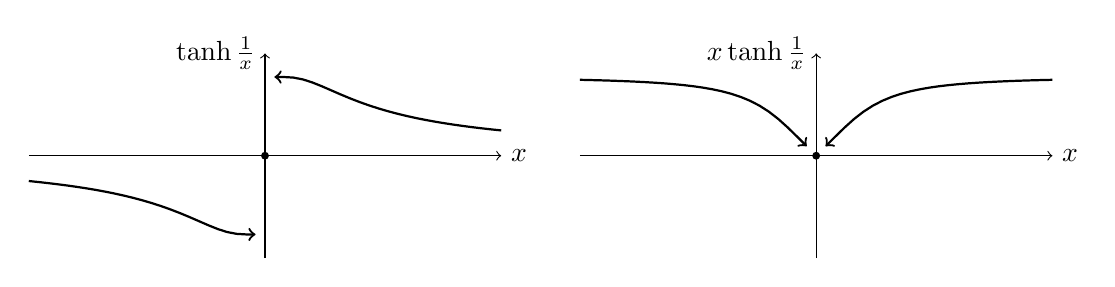
\begin{tikzpicture}
\pgfmathsetmacro{\a}{3};
\pgfmathsetmacro{\e}{0.12};
\draw[ ->] (-\a,0)--(\a,0)node[right]{$x$};
\draw[ ->] (0,-1.3)--(0,1.3)node[left]{$\tanh\frac1x$};
\draw[->, thick, domain=-\a:-\e] plot (\x,
{(exp(1/\x)-exp(-1/\x))/(exp(1/\x)+exp(-1/\x))});
\draw[<-, thick, domain=\e:\a] plot (\x, {(exp(1/\x)-exp(-1/\x))/(exp(1/\x)+exp(-1/\x))});
\fill (0,0) circle (0.50mm);

\begin{scope}[xshift=7cm]
\draw[ ->] (-\a,0)--(\a,0)node[right]{$x$};
\draw[ ->] (0,-1.3)--(0,1.3)node[left]{$x\tanh\frac1x$};
\draw[->, thick, domain=-\a:-\e] plot (\x,
{\x*(exp(1/\x)-exp(-1/\x))/(exp(1/\x)+exp(-1/\x))});
\draw[<-, thick, domain=\e:\a] plot (\x,
{\x*(exp(1/\x)-exp(-1/\x))/(exp(1/\x)+exp(-1/\x))});
\fill (0,0) circle (0.50mm);
\end{scope}
\end{tikzpicture}\end{bmlimage}
\end{center}
\end{sol}
\end{exo}


\section{O Teorema do valor intermediário}
\index{Teorema!do valor intermediário}
Funções contínuas possuem propriedades muito particulares.
Considere por exemplo
uma função contínua num intervalo fechado, $f:[a,b]\to \bR$. 
Então, ao $x$ variar entre $a$ e $b$, \emph{o gráfico de $f$ corta 
qualquer reta horizontal
intermediária, de altura $h$ entre $f(a)$ e $f(b)$, pelo menos uma
vez}:

\begin{center}
\begin{bmlimage}\begin{tikzpicture}
\pgfmathsetmacro{\taille}{6};
\pgfmathsetmacro{\N}{200};
\pgfmathsetmacro{\incrx}{\taille/\N};
\pgfmathsetmacro{\incry}{3/sqrt(\N)};
\pgfmathsetmacro{\a}{1};
\pgfmathsetmacro{\b}{6};


\pgfmathsetmacro{\m}{-40};
\pgfmathsetmacro{\n}{20};
\pgfmathsetmacro{\o}{30};
\pgfmathsetmacro{\p}{65};
\pgfmathsetmacro{\q}{18};
\pgfmathsetmacro{\r}{-10};

\coordinate (A) at (1,0.5);
\coordinate (B) at (6,3);
\coordinate (C) at (4,2);

\draw[dotted] (1,0)node[below]{$a$}--(A)--(0,0.5)
node[left]{$f(a)$};
\draw[dotted] (6,0)node[below]{$b$}--(B)--(0,3)
node[left]{$f(a)$};
\draw (0,2)node[left]{$h$} -- (6,2);
\draw[dashed] (4,0)node[below]{$c$} -- (C);

\fill (A) circle (0.50mm);
\fill (B) circle (0.50mm);
\fill (C) circle (0.50mm);

\draw[thick] 
(A) to[out=\m, in={180+\n}] 
(2,0.2) to[out=\n, in={180+\o}] 
(3,1.2) to[out=\o, in={180+\p}] 
(C) to[out=\p, in={180+\q}] 
(5,3.7) to[out=\q, in={180+\r}] 
(B);


%\draw (A) .. controls (-1,-1) .. (B);
%\draw (A) .. controls (1,1) .. (B);
%\draw (0,0) .. controls (1,1) .. (4,0)
%      (5,0) .. controls (6,0) and (6,1) .. (5,2);
%\coordinate (origin) at (\x,\y);
%\coordinate (current) at (origin);

%\foreach \k in {1,...,\N} {
%\draw[thick] (current)-- ++ (\incrx,{(2*rnd-0.91)*\incry}) coordinate (current); 
%\pgfmathtruncatemacro{\NN}{\N/2};
%\ifnum \k=\NN  
%\coordinate (currentVV) at ($(0,-10)!(current)!(0,10)$);
%\coordinate (currentVVV) at ($({\x+\taille},-10)!(current)!({\x+\taille},10)$);
%\coordinate (currentHH) at ($(0,0)!(current)!(2*\taille,0)$);
%\draw[dashed] (currentVV)node[left]{$h$}--(currentVVV);
%\draw[dotted] (current)--(currentHH)node[below]{$c$};
%\fill (current) circle (0.60mm);
%\fi
%}
%
%\coordinate (currentV) at ($(\x,-10)!(current)!(\x,10)$);
%\coordinate (currentVV) at ($(0,-10)!(current)!(0,10)$);
%\coordinate (currentH) at ($(origin)!(current)!(2*\taille,\y)$);
%
%\fill (origin) circle (0.50mm);
%\fill (current) circle (0.50mm);
%
%\draw[dotted] (\x,0)node[below]{$a$}--(origin);
%\draw[dotted] (\x+\taille,0)node[below]{$b$}--(current);
%\draw[dashed] (0,\y)node[left]{$\scriptstyle{f(a)}$}--({\x+\taille},\y);
%\draw[dashed] (currentVV)node[left]{$\scriptstyle{f(b)}$}--(current);
\draw[ ->] (-0.5,0)--(\taille+2,0)node[right]{$x$};
\draw[ ->] (0,-0.5)--(0,3.5) node[right]{$f(x)$};

\end{tikzpicture}\end{bmlimage}
\end{center}

\begin{teo}[Teorema do Valor Intermediário]\label{Teo:ValInterm}
Seja  $f:[a,b]\to \bR$ uma função contínua, tal que $f(a)<f(b)$. 
Então para todo $h\in [f(a),f(b)]$, existe $c\in [a,b]$ tal que
$f(c)=h$. Uma afirmação parecida vale quando $f(a)>f(b)$
\end{teo}

\begin{exo}
Para cada função abaixo, estude a propriedade do valor
intermediário (isto é, fixe uma reta de altura $h$ e vê se o gráfico de $f$
corta a reta).
%\begin{multicols}{2}
\begin{enumerate}
\item $f:[-1,2]\to \bR$, $f(x)\pardef x^2$.
\item $g:[-1,1]\to \bR$, 
$g(x)\pardef
\begin{cases}
\frac{|x|}{x}&\text{ se }x\neq 0\,,\\
0&\text{ se }x=0\,.\\
\end{cases}
$
\item $h:[0,2]\to \bR$, 
$h(x)\pardef
\begin{cases}
2x-1&\text{ se }0\leq x<1\,,\\
2x-3&\text{ se }1\leq x\leq 2\,.\\
\end{cases}
$
\end{enumerate}
%\end{multicols}
\begin{sol}
(Esboçar os gráficos de $f,g,h$ ajuda a compreensão do exercício).

Temos $f(-1)=1$, $f(2)=4$.
Como $f$ é contínua, o Teorema \eqref{Teo:ValInterm} se aplica:
se $1\leq h\leq 4$, o gráfico de $f$ corta a reta horizontal de
altura $y=h$ pelo menos uma vez. Na verdade, ele corta a reta
exatamente uma vez se $1<h\leq 4$, e duas vezes se $h=1$.

Temos $g(-1)=-1$, $g(1)=1$. 
Como $g$ é descontínua em $x=0$, o teorema não se aplica. Por
exemplo, o gráfico de $g$ nunca corta a reta horizontal $y=\frac12$.

Temos $h(0)=-1$, $h(2)=1$. Apesar de $h$ não ser contínua, ela
satisfaz à propriedade do valor intermediário. De fato, o gráfico de
$h$ corta a reta $y=h_*$ duas vezes se $-1\leq h_*<1$, e uma vez se $h_*=1$.
\end{sol}
\end{exo}

O Teorema do valor intermediário pode ser usado para 
a resolução numérica de equações:

\index{resolução numérica}
\begin{ex}
Considere a função 
$f(x)\pardef \tfrac12-x^2-x^5$,
no intervalo $[-1,1]$. Como $f$ é contínua e muda de
sinal entre $-1$ e $+1$,
$f(-1)=\frac12>0$, 
$f(+1)=-\frac32<0$, 
o Teorema do Valor Intermediário implica que 
deve existir pelo menos um ponto $x_*\in [-1,1]$ tal que $f(x^*)=0$.
\begin{center}
\begin{bmlimage}\begin{tikzpicture}[scale=1.7]
%\draw[very thin, gray] (0,0) grid[step=0.1] (5,2);
\newcommand{\funcao}[1]{0.5-(#1)^2-(#1)^5}
\draw[ ->] (-1.5,0)--(1.5,0) node[right]{$x$};
\draw[ ->] (0,-1.2)--(0,1.3) node[right]{$f(x)$};
\draw[thick, domain=-1:1, samples=100] plot (\x,{\funcao{\x}});
\draw[dotted] (-1,0)node[below]{$-1$}--(-1,{\funcao{-1}});
\fill (-1,{\funcao{-1}}) circle (0.45mm);
\draw[dotted] (1,0)node[above]{$+1$}--(1,{\funcao{1}});
\fill (1,{\funcao{1}}) circle (0.45mm);
\coordinate (a) at (0.622,0);
\fill (a) circle (0.45mm);
\draw (a) node[below left]{$x_*$};
\end{tikzpicture}\end{bmlimage}
\end{center}

Como calcular $x_*$? Por definição, $x_*\in [-1,1]$ é solução da
equação do quinto grau:
$$x^5+x^2-\tfrac12=0\,,$$
Como não existe um método geral para a resolução de tais equações, vejamos um
método que, sem ser \emph{exato}, fornece pelo menos uma \emph{aproximação}
de $x_*$.\\

A ideia é de localizar $x_*$ usando recursivamente o Teorema do Valor intermediário. 
Para começar, observemos que como $f(0)>0$, $f(1)<0$, 
$f$ muda de sinal também no intervalo $[0,1]$, o que implica que 
$x_*\in [0,1]$.\\

Calculemos então o valor de $f$ no meio do
intervalo $[0,1]$ e observemos que $f(\frac12)>0$. Portanto, $f$ muda
de sinal entre $\frac12$ e $1$, o que implica que $x_*\in
[\frac12,1]$. 
Em seguida, $f(\frac34)<0$ implica que $f$ muda de sinal entre
$\frac12$ e $\frac34$, isto é, $x_*\in [\frac12,\frac34]$. Continuando
assim, obtemos uma sequência decrescente de intervalos encaixados,
cada um contendo $x_*$:
$$[0,1]\supset [\tfrac12,1]\supset [\tfrac12,\tfrac34]\supset \cdots
$$
Os tamanhos dos intervalos decrescem exponencialmente rápido: o
primeiro tem tamanho $1$, o segundo tamanho $\frac12$, etc., o 
$n$-ésimo tem tamanho $2^{-n}$.
Logo, qualquer ponto do $n$-ésimo intervalo dá uma aproximação 
de $x_*$ com uma precisão de $2^{-n}$.\\

O método descrito acima, que consiste em usar o Teorema do Valor
intermediário a cada etapa, é chamado de \emph{método da bisseção}.

\end{ex}




\section{Limites e funções contínuas}\label{Sec:FuncConteLim}
\index{limites!de funções contínuas}
%Uma função $f$ ser contínua implica que se $x\to a$, então $f(x)\to f(a)$.
Como visto na Proposição \ref{Prop:continuidadechiante}, se 
$g$ é contínua em $a$, e se $f$ é contínua em $g(a)$, então $f\circ g$ é
contínua em $a$. Isso pode ser dito da seguinte maneira: \emph{se $g(x)\to L$
quando $x\to a$ e se $f$ é contínua em $L$, então $f(g(x))\to f(L)$ quando
$x\to a$.} Isto é,
$$\lim_{x\to a}f(g(x))= f\bigl(\lim_{x\to a}g(x)\bigr)\,.$$
Esse fato foi usado, sem sequer ser mencionado, em vários lugares nas seções
anteriores. Por exemplo apareceu, no item \eqref{itexosinxx5}
do Exercício \ref{Exo:variantessinxsurx}, o limite de $(\frac{\sen
x}{x})^2$ quando $x\to 0$. Aqui, a função é da forma $f(g(x))$, com
$g(x)=\frac{\sen x}{x}$, $f(x)=x^2$. Ora, como $g(x)\to 1$ e como $f$ é
contínua em $1$, podemos ``entrar o limite dentro do $(\cdot)^2$'':
$$
\lim_{x\to 0}\Bigl(
\frac{\sen x}{x}
\Bigr)^2=\Bigl(\lim_{x\to 0}
\frac{\sen x}{x}
\Bigr)^2=(1)^2=1\,.
$$
Também, no item \eqref{itexolimelem20} do Exercício
\ref{Exo:Limiteselementares}, como $\sqrt{x}$ é contínua a direita em $0$
$$
\lim_{x\to 1^+}\sqrt{\ln x}=\sqrt{\lim_{x\to 1^+}{\ln x}}=\sqrt{0}=0\,.
$$
Um resultado parecido vale para limites no infinito:  \emph{se $g(x)\to L$
quando $x\to \infty$ e se $f$ é contínua em $L$, então $f(g(x))\to f(L)$
quando $x\to \infty$.} Em outras palavras:
$$\lim_{x\to \infty}f(g(x))= f\bigl(\lim_{x\to \infty}g(x)\bigr)\,.$$
Por exemplo, em \eqref{eq:usoimpliccontinlog}, 
\eq{\label{eq:usoimpliccontinlogBIS}
\lim_{z\to+\infty}\ln\bigl((1+\tfrac{1}{z})^z\bigr)
=\ln\Bigl(\lim_{z\to+\infty}(1+\tfrac{1}{z})^z\Bigr)
=\ln e=1\,.
}

%\newpage
\section{Exercícios de revisão}

\begin{exo}
Considere 
$$
f(x)\pardef
\begin{cases}
\sqrt{x^4+1}-(ax^2+b)+\frac{1-\cos (cx)}{x^2} &\text{ se }x\neq 0 \,,\\
0  & \text{ se }x=0\,.
\end{cases}
$$
Ache $a,b,c$ de modo tal que $f$ seja contínua em $0$, e que $\lim_{x\to \infty}=-3$.
\begin{sol}
$a=1$, $b=3$, $c=\pm 2$.
\end{sol}
\end{exo}


\begin{exo}
Seja $f:\bR\to \bR$ contínua tal que $\lim_{x\to +\infty}f(x)=+\infty$,
$\lim_{x\to -\infty}f(x)=-\infty$. Mostre que $\imagem(f)=\bR$.
\begin{sol}
Seja $y\in \bR$ fixo, qualquer. Como $\lim_{x\to
+\infty}f(x)=+\infty$, existe $b>0$ grande o suficiente tal que
$f(b)>y$. 
Como $\lim_{x\to -\infty}f(x)=-\infty$, existe $a<0$ grande o
suficiente tal que $f(a)<y$. 
Pelo Teorema do Valor Intermediário, existe $c\in [a,b]$ tal que
$f(c)=y$. Isto implica que $y\in \imagem(f)$.
\end{sol}
\end{exo}


\begin{exo}
Se $f$ é par (respectivamente ímpar), qual é a relação entre 
$\lim_{x\to 0^+}f(x)$ e $\lim_{x\to 0^-}f(x)$?
Seja $f$ uma função ímpar tal que $\lim_{x\to 0^+}f(x)$ existe e vale $L>0$.
Essa função é contínua?
\begin{sol}
Considere $\lim_{x\to 0^-}f(x)$. Chamando $y\pardef -x$, $x\to 0^-$ corresponde
a $y\to 0^+$.
Logo, $$\lim_{x\to 0^-}f(x)=\lim_{y\to 0^+}f(-y)=-\lim_{y\to 0^+}f(y)\equiv-
\lim_{x\to 0^+}f(x)\,.$$
Portanto, para uma função ímpar ser contínua em $0$, é preciso ter 
$\lim_{x\to 0^+}f(x)=f(0)=0$ (não pode ser $L>0$).
\end{sol}
\end{exo}

\begin{exo} (Aplicação do Teorema do valor Intermediário).
Se $I$ é um intervalo e se $f:I\to \bR$ é contínua, então
$\imagem(f)$ é um
intervalo.
\end{exo}



\begin{exo}
Estude a continuidade das seguintes funções:
$$
f(x)\pardef 
\begin{cases}
 e^{\arctan 1/x}&\text{se }x\neq 0\,,\\
e^{\frac{\pi}{2}}&\text{ se }x=0\,,
\end{cases}
\quad\quad
g(x)\pardef 
\begin{cases}
 e^{\frac{x}{x^2-1}}&\text{se }x\not\in \{\pm 1\}\,,\\
0&\text{se }x=-1\,,\\
1&\text{se }x=+1\,.
\end{cases}
$$
% \begin{sol}
% Como $\frac{1}{x}$ é contínua em qualquer $a\neq 0$, que $\arctan x$ é
%contínua 
% em $\frac{1}{a}$, e que $e^x$ é contínua em $\arctan \frac1a$, temos
%que 
% $f(x)$ é contínua em qualquer $a\neq 0$. Em $a=0$ temos:
% $$
% \lim_{x\to 0^\pm }f(x)=\lim_{x\to 0^\pm}e^{\arctan 1/x}
% =e^{\lim_{x\to 0^\pm}\arctan 1/x}=e^{\arctan(\lim_{x\to 0^\pm}
% 1/x)}=e^{\pm\frac{\pi}{2}}\,.
% $$
% Logo $f$ é contínua a direita (mas descontínua) em $0$.
% Por outro lado, $g$ é contínua em qualquer $x\neq \pm 1$, e descontínua em
% $x=\pm 1$.
% \end{sol}
\end{exo}

\begin{exo}
Sejam $f,g$ duas funções contínuas na reta, tais que $f(x)=g(x)$ para todo
racional diádico $x$. Mostre que $f=g$.
\end{exo}



